%%%%%%%%%%%%%%%%%%%%%%%%%%%%%%%%%%%%%%%%%
% Masters/Doctoral Thesis 
% LaTeX Template
% Version 2.4 (22/11/16)
%
% This template has been downloaded from:
% http://www.LaTeXTemplates.com
%
% Version 2.x major modifications by:
% Vel (vel@latextemplates.com)
%
% This template is based on a template by:
% Steve Gunn (http://users.ecs.soton.ac.uk/srg/softwaretools/document/templates/)
% Sunil Patel (http://www.sunilpatel.co.uk/thesis-template/)
%
% Template license:
% CC BY-NC-SA 3.0 (http://creativecommons.org/licenses/by-nc-sa/3.0/)
%
%%%%%%%%%%%%%%%%%%%%%%%%%%%%%%%%%%%%%%%%%

%----------------------------------------------------------------------------------------
%	PACKAGES AND OTHER DOCUMENT CONFIGURATIONS
%----------------------------------------------------------------------------------------

\documentclass[
11pt, % The default document font size, options: 10pt, 11pt, 12pt
oneside, % Two side (alternating margins) for binding by default, uncomment to switch to one side
english, % ngerman for German
%singlespacing, % Single line spacing, alternatives: onehalfspacing or doublespacing
onehalfspacing, % Single line spacing, alternatives: onehalfspacing or doublespacing
%draft, % Uncomment to enable draft mode (no pictures, no links, overfull hboxes indicated)
nolistspacing, % If the document is onehalfspacing or doublespacing, uncomment this to set spacing in lists to single
%liststotoc, % Uncomment to add the list of figures/tables/etc to the table of contents
%toctotoc, % Uncomment to add the main table of contents to the table of contents
%parskip, % Uncomment to add space between paragraphs
%nohyperref, % Uncomment to not load the hyperref package
hidelinks, %To remove colored links
headsepline, % Uncomment to get a line under the header
%chapterinoneline, % Uncomment to place the chapter title next to the number on one line
consistentlayout, % Uncomment to change the layout of the declaration, abstract and acknowledgements pages to match the default layout
table, %for xcolor
]{MastersDoctoralThesis} % The class file specifying the document structure

\usepackage[utf8]{inputenc} % Required for inputting international characters
\usepackage[T1]{fontenc} % Output font encoding for international characters

\usepackage[titletoc]{appendix}

\usepackage{palatino} % Use the Palatino font by default

\usepackage{textcomp} %copyright

\usepackage{listings} %for code highlighting

\usepackage{amsmath}

\usepackage{tikz}

\usepackage[backend=bibtex,style=ieee,natbib=true]{biblatex} % Use the bibtex backend with the authoryear citation style (which resembles APA)

\usepackage[]{siunitx} %for SI units

\addbibresource{main.bib} % The filename of the bibliography

\usepackage[autostyle=true]{csquotes} % Required to generate language-dependent quotes in the bibliography

%\usepackage{color, colortbl} % For colored tables

\definecolor{Gray}{gray}{0.925}
\definecolor{Transparent}{gray}{1}

%----------------------------------------------------------------------------------------
%	MARGIN SETTINGS
%----------------------------------------------------------------------------------------

\geometry{
	paper=a4paper, % Change to letterpaper for US letter
	inner=2.5cm, % Inner margin
	outer=3.8cm, % Outer margin
	bindingoffset=.5cm, % Binding offset
	top=1.5cm, % Top margin
	bottom=1.5cm, % Bottom margin
	%showframe, % Uncomment to show how the type block is set on the page
}

%----------------------------------------------------------------------------------------
%	THESIS INFORMATION
%----------------------------------------------------------------------------------------

\thesistitle{Augmented Reality with Location Tracking} % Your thesis title, this is used in the title and abstract, print it elsewhere with \ttitle
\supervisor{Dr. Robert McLeod \\ Dr. Ekram Hossain} % Your supervisor's name, this is used in the title page, print it elsewhere with \supname
\examiner{} % Your examiner's name, this is not currently used anywhere in the template, print it elsewhere with \examname
\degree{Bachelor of Science} % Your degree name, this is used in the title page and abstract, print it elsewhere with \degreename
\author{Drew Barclay \\ Maricar Aliasut \\ Llandro Ojeda} % Your name, this is used in the title page and abstract, print it elsewhere with \authorname
\addresses{} % Your address, this is not currently used anywhere in the template, print it elsewhere with \addressname

\subject{Biological Sciences} % Your subject area, this is not currently used anywhere in the template, print it elsewhere with \subjectname
\keywords{} % Keywords for your thesis, this is not currently used anywhere in the template, print it elsewhere with \keywordnames
\university{\href{http://umanitoba.ca/}{University of Manitoba}} % Your university's name and URL, this is used in the title page and abstract, print it elsewhere with \univname
\department{\href{http://umanitoba.ca/faculties/engineering/departments/ece/}{Electrical \& Computer Engineering}} % Your department's name and URL, this is used in the title page and abstract, print it elsewhere with \deptname
\group{Group 20} % Your research group's name and URL, this is used in the title page, print it elsewhere with \groupname
\faculty{\href{http://umanitoba.ca/faculties/engineering/index.html}{Faculty of Engineering}} % Your faculty's name and URL, this is used in the title page and abstract, print it elsewhere with \facname

\AtBeginDocument{
\hypersetup{pdftitle=\ttitle} % Set the PDF's title to your title
\hypersetup{pdfauthor=\authorname} % Set the PDF's author to your name
\hypersetup{pdfkeywords=\keywordnames} % Set the PDF's keywords to your keywords
%\hypersetup{colorlinks=false}
\hypersetup{hidelinks=true}
}

\begin{document}

\frontmatter % Use roman page numbering style (i, ii, iii, iv...) for the pre-content pages

\pagestyle{plain} % Default to the plain heading style until the thesis style is called for the body content

%----------------------------------------------------------------------------------------
% COMMANDS
%----------------------------------------------------------------------------------------

% Define some commands to keep the formatting separated from the content 
\newcommand{\keyword}[1]{\textbf{#1}}
\newcommand{\tabhead}[1]{\textbf{#1}}
\newcommand{\code}[1]{\texttt{#1}}
\newcommand{\file}[1]{\texttt{\bfseries#1}}
\newcommand{\option}[1]{\texttt{\itshape#1}}

%----------------------------------------------------------------------------------------
%	TITLE PAGE
%----------------------------------------------------------------------------------------

\begin{titlepage}
\begin{center}

\vspace*{.06\textheight}
%{\scshape\LARGE \univname\par}\vspace{1.5cm} % University name
\textsc{\Large Capstone Project Final Report}\\[0.5cm] % Thesis type

\HRule \\[0.4cm] % Horizontal line
{\huge \bfseries \ttitle\par}\vspace{0.4cm} % Thesis title
\HRule \\[1.5cm] % Horizontal line
 
\begin{minipage}[t]{0.4\textwidth}
\begin{flushleft} \large
\emph{Authors:}\\
{\authorname} % Author name - remove the \href bracket to remove the link
\end{flushleft}
\end{minipage}
\begin{minipage}[t]{0.4\textwidth}
\begin{flushright} \large
\emph{Advisors:} \\
{\supname} % Supervisor name - remove the \href bracket to remove the link  
\end{flushright}
\end{minipage}\\[3cm]
 
\vfill

\large \textit{Final report submitted in partial satisfaction of the requirements for the degree of \degreename}\\[0.3cm] % University requirement text
\textit{in}\\[0.4cm]
\deptname\\[0.4cm] % Research group name and department name
\textit{in the}\\[0.4cm]
\facname \\[0.4cm]
\textit{of the}\\[0.4cm]
\univname\\
 
\vspace*{\fill}

{\large Spring 2017}\\

{\small \textcopyright \, Copyright by Drew Barclay, Maricar Aliasut, Llandro Ojeda, 2017}\\
%{\large \today}\\[4cm] % Date
%\includegraphics{Logo} % University/department logo - uncomment to place it
 
\vfill
\end{center}
\end{titlepage}

%----------------------------------------------------------------------------------------
%	ABSTRACT PAGE
%----------------------------------------------------------------------------------------

\begin{abstract}
\addchaptertocentry{\abstractname} % Add the abstract to the table of contents
•  Statement of the problem

•  Procedures and methods used

•  Results and Conclusions
\end{abstract}

%----------------------------------------------------------------------------------------
%	ACKNOWLEDGEMENTS
%----------------------------------------------------------------------------------------

\begin{acknowledgements}
\addchaptertocentry{\acknowledgementname} % Add the acknowledgements to the table of contents
This project would not have been possible without a lot of people:

\begin{itemize}
	\item Our advisors, Dr. Ekram Hossain and Dr. Bob McLeod for taking us on despite having a risky project. Bob McLeod's generous financial support was a great help as well.
	\item Zoran Trajkoski, for helping us learn to solder (and for doing a lot of the soldering, saving us hours of time).
	\item Derek Oliver for allowing us to form a group of three, rather than the minimum of four normally required. 
	\item Aidan Topping for reading over the report and offering suggestions.
	\item Thomas ``thotro'' Trojer for his arduino-dw1000 project on Github, which allowed us to quickly determine whether we could do the project at all.
	\item Aleksandar ``d3alek'' Kodzhabashev and fractious for their work on the Texample2 3D text rendering library we used.
\end{itemize}

Thank you all.
\end{acknowledgements}

\begin{contributions}
\addchaptertocentry{\contributionsname} % Add the acknowledgements to the table of contents

There were three main facets to the technical side of the project: rangefinding, position calculation, and augmented reality. On the management side of the project, there were the oral and written reports, and the project proposal.

\begin{table}[ht]
\centering
\begin{tabular}{ l | c | c | c }
  \toprule
   \tabhead{Task} & \tabhead{Drew} & \tabhead{Maricar} & \tabhead{Llandro} \\
   \midrule
   \rowcolor{Gray}
  \tabhead{Research} & & & \\
  ~~Bluetooth Rangefinding & \textbullet & & \\
  ~~Google Cardboard & & \textbullet &  \\
  ~~DWM1000 and Arduino Code & & & \textbullet \\
  \midrule
  \rowcolor{Gray}
  \tabhead{Rangefinding} & & & \\
  ~~PCB Design & \textbullet & &  \\
  ~~Soldering & \textbullet & & \textbullet  \\
  ~~Software & \textbullet && \\
  \midrule
  \rowcolor{Gray}
  \tabhead{Position Calculation} & & & \\
  ~~Math & \textbullet & & \textbullet \\
  ~~Coding & \textbullet & & \\
  \midrule
  \rowcolor{Gray}
  \tabhead{Augmented Reality} & & & \\
  ~~Camera Capture & \textbullet & \textbullet & \textbullet \\
  ~~3D Graphics & \textbullet & & \\
  ~~Graphical Assets & & \textbullet & \\
  \midrule
  \rowcolor{Gray}
  \tabhead{Administration} & & & \\
  ~~Design Proposal (Oral) & & \textbullet  & \\
  ~~Design Proposal (Written) & \textbullet & \textbullet & \textbullet \\
  ~~Design Review 2 & & & \textbullet \\
  ~~Design Review 3 & \textbullet & & \\
  ~~Design Review 4 & \textbullet & & \\
  ~~Final Report & \textbullet & \textbullet & \textbullet \\
  ~~Final Presentation & \textbullet & \textbullet & \textbullet \\
  \bottomrule
  
\end{tabular}
\end{table}

\end{contributions}


%----------------------------------------------------------------------------------------
%	LIST OF CONTENTS/FIGURES/TABLES PAGES
%----------------------------------------------------------------------------------------

\tableofcontents % Prints the main table of contents

\listoffigures % Prints the list of figures

\listoftables % Prints the list of tables

%----------------------------------------------------------------------------------------
%	ABBREVIATIONS
%----------------------------------------------------------------------------------------

\begin{abbreviations}{ll} % Include a list of abbreviations (a table of two columns)

\textbf{PCB} & Printed circuit board. \\
\textbf{UWB} & Ultra-wideband. A type of radio technology. \\

\end{abbreviations}

%----------------------------------------------------------------------------------------
%	PHYSICAL CONSTANTS/OTHER DEFINITIONS
%----------------------------------------------------------------------------------------

\begin{constants}{lr@{${}={}$}l} % The list of physical constants is a three column table

% The \SI{}{} command is provided by the siunitx package, see its documentation for instructions on how to use it

Speed of Light & $c_{0}$ & \SI{2.99792458e8}{\meter\per\second} (exact)\\
%Constant Name & $Symbol$ & $Constant Value$ with units\\

\end{constants}

%----------------------------------------------------------------------------------------
%	SYMBOLS
%----------------------------------------------------------------------------------------

\begin{symbols}{lll} % Include a list of Symbols (a three column table)

$a$ & distance & \si{\meter} \\
$P$ & power & \si{\watt} (\si{\joule\per\second}) \\
%Symbol & Name & Unit \\

\addlinespace % Gap to separate the Roman symbols from the Greek

$\omega$ & angular frequency & \si{\radian} \\

\end{symbols}

%----------------------------------------------------------------------------------------
%	DEDICATION
%----------------------------------------------------------------------------------------

%\dedicatory{For/Dedicated to/To my\ldots} 

%----------------------------------------------------------------------------------------
%	THESIS CONTENT - CHAPTERS
%----------------------------------------------------------------------------------------

\mainmatter % Begin numeric (1,2,3...) page numbering

\pagestyle{thesis} % Return the page headers back to the "thesis" style

% Include the chapters of the thesis as separate files from the Chapters folder
% Uncomment the lines as you write the chapters

% Introduction

\chapter{Introduction} % Main chapter title

\label{Introduction} % For referencing the chapter elsewhere, use \ref{Chapter1} 

%----------------------------------------------------------------------------------------

\section{Motivation}

Valve recently released SteamVR which is to work with the HTC Vive in order to promote virtual reality in their games. Videogames are the platform for interactive media. In the last few years, starting with Nintendo’s Wii console, companies have started to heavily invest in developing ways for users to interact more intimately with their media, where they become ``one with the game”.

This movement started with the introduction of \emph{Star Trek}’s holodeck and \emph{X-Men}’s Danger Room, which use holographic images to create another reality within a room. This project is in some ways the opposite of that; the ``game'' is inserted into real life. The game is “augmented” into the current time and place, hence the term \textbf{augmented reality} (AR). Augmented reality is where portions of a graphical user interface from a program is seen in the eyes of a user right then and there through a \textbf{heads up display} (HUD). It is heavily inspired by many first person shooter videogames such as \emph{Halo} and \emph{Call of Duty}. 

Augmented reality can be used in many applications, from a surgeon seeing detailed vital signs of a patient to a soldier keeping track of his teammates. This project looks at a practical application of tracking locations of objects and displaying them on a HUD.

\section{System Overview}

\begin{figure}
	\centering
	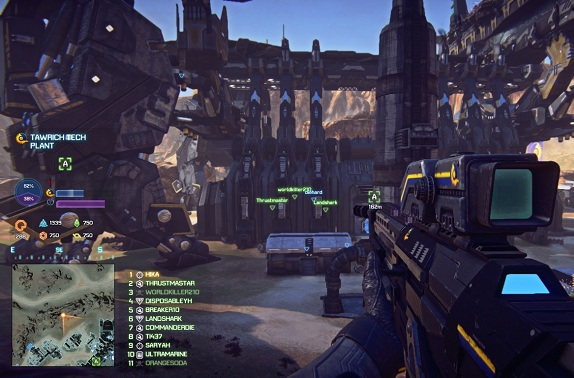
\includegraphics[width=\linewidth]{Figures/GameHUD.jpg}
	\decoRule
	\caption{A screenshot of the videogame \emph{Planetside 2}, showing its HUD. Locations of objectives and allies are indicated with triangles.}
	\label{fig:GameHUD}
\end{figure}

\begin{figure}
	\centering
	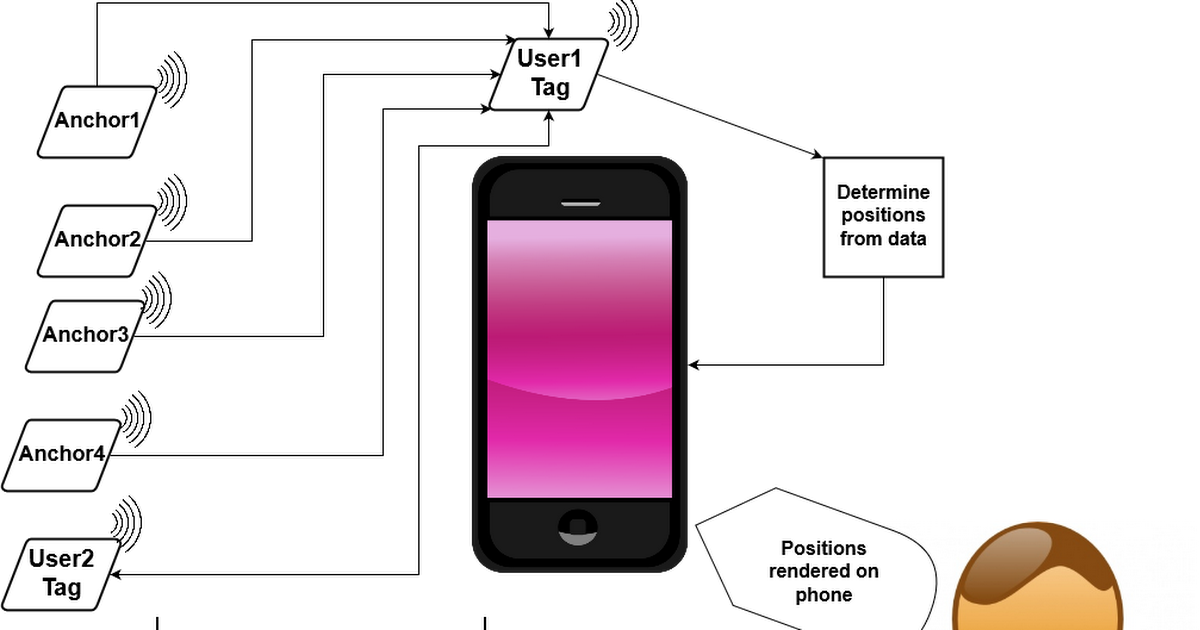
\includegraphics[width=\linewidth]{Figures/ARBlockDiagram.png}
	\decoRule
	\caption{A system block diagram of the project.}
	\label{fig:SystemBlockDiagram}
\end{figure}

This project takes the visual HUD very popular in video games such as \emph{Planetside 2}, as seen in Figure~\ref{fig:GameHUD}, and reproduces it for use in the actual real world.  While there are many applications and ideas for a heads up display, the project is focused on a proof of concept locating and tracking certain objects within the display. With further development and investment, the project could be expanded and improved upon for many applications. For example, keeping track of a person’s pulse while a surgeon is performing surgery or the marking of a driver's destination on their windshield.

To locate a target, devices called tags are used to mark objects or locations of interest. Each tag is affixed to the target that is to be tracked. The tags determine their distances to other tags, and these distances are triangulated and the positions of tracked objects determined. For 3D positioning, a minimum of four tags are necessary to precisely pinpoint an object's location. This is shown in Figure~\ref{fig:SystemBlockDiagram}.

There are three main parts to this project: 
\begin{itemize}
	\item \textbf{Rangefinding} (Chapters~\ref{Rangefinding} and \ref{RangefindingHardware}). Rangefinding uses tags to determine the ranges (distances) between other tags.
	\item \textbf{Position Calculation} (Chapter \ref{PositionCalculation}). Position calculation involves processing the range data from the tags to produce positions in 3D space for use within the augmented reality portion of the project.
	\item \textbf{Augmented Reality Rendering} (Chapter \ref{AugmentedReality}). The AR subsystem marks the locations of tracked targets on the screen of a cellphone.
\end{itemize}


% Rangefinding

\chapter{Rangefinding} % Main chapter title

\label{Rangefinding}

%----------------------------------------------------------------------------------------

\section{Overview}
 Rangefinding is the act of determining the distance between two things.
 
\subsection{The System}

\begin{figure}
	\centering
	\tikzstyle{vertex}=[circle, draw]
\begin{tikzpicture}[transform shape]
\node[vertex](a1) at (0, 0) {$ a_1 $};
\node[vertex](a2) at (3, 3) {$ a_2 $};
\node[vertex](a3) at (6, 0) {$ a_3 $};
\node[vertex](t1) at (-3,1.5) {$ t_1 $};

\begin{scope}[every path/.style={-}, every node/.style={inner sep=1pt}]
       \draw (a1) -- node [anchor=south east] {$4$} (a2);
       \draw (a2) -- node [anchor=south west] {$4$} (a3);
       \draw (a1) -- node [anchor=north] {$6$} (a3);
       \draw (t1) -- node [anchor=north east] {$5.4$} (a1);
       \draw (t1) -- node [anchor=south east] {$6.2$} (a2);
       \draw (t1) -- node [pos=0.2, anchor=south west] {$9.1$} (a3);
\end{scope} 
\end{tikzpicture}
	\decoRule
	\caption{An example network, showing 1 tag $t_1$ and 3 anchors $a_i$ and the reported distances between them. Note that each device calculates its own range to the other devices, which will be slightly different from the range calculated on the other devices. This is not shown on the diagram.}
	\label{fig:ExampleNetwork}
\end{figure}

The rangefinding subsystem is comprised of \textbf{nodes} in a network, each of which is capable of sending and receiving wireless signals.

Each node is either an \textbf{anchor} or a \textbf{tag}. Both tags and anchors use essentially the same hardware and code, but anchors are assumed to be stationary while tags are mobile. Stationary nodes are required so as to provide a consistent frame of reference for other nodes when calculating positions later on. More information on this can be found in Section~\ref{FrameOfReference}.

The rangefinding subsystem's purpose is to determine the distances between every pair of nodes in the network. With this data, the position calculation subsystem can then determine the positions of every anchor and tag in 3D space. An example 2D rangefinding network is shown in Figure~\ref{fig:ExampleNetwork}.

\subsection{Rangefinding}
Rangefinding is done wirelessly. The underlying concept is that if we precisely note the times at which we send and receive a signal, then -- since light travels at a fixed speed -- we can determine the distance the signal traveled, which is the distance between the nodes. 

The basic algorithm for the network is: 
\begin{enumerate}
	\item Each node broadcasts a message to every other node, and every node responds. 
	\item The time it took for the message to travel from one node to another and then back (minus the time spent processing the received messages) is calculated.
	\item With some simple math involving the speed of light the distance between the nodes is calculated. 
\end{enumerate}

This method of calculating range is known as \textbf{time-of-flight} (TOF).

Each node is comprised of a DWM1000, can send wireless signals, and an Arduino microcontroller.

\subsection{Requirements}
There are a number of useful characteristics a rangefinding system should have:
\begin{itemize}
	\item Ranges should be accurate and not very noisy.
	\item Ranges should be calculated at a high frequency. If they are not, then we cannot calculate positions quickly and moving objects will have their positions displayed inaccurately.
	\item The system should be able to cover a large area. 
	\item The system should be robust to nodes entering/leaving the network. 
\end{itemize}

It will be demonstrated how we sought to satisfy these criteria.

(TODO TALK ABOUT WHAT IS COMING UP IN THE REST OF THE CHAPTER)

\section{Time-of-Flight}
This section briefly covers the math behind time-of-flight range calculations. For more in-depth information, \parencite{DW1000UserManual} has a comprehensive write-up of the different ways wireless ranging can be performed as well as an error analysis.

\subsection{Propagation Time}
The goal behind time-of-flight is to measure the propagation time of a signal, $T_{prop}$. Once we obtain this, it is a simple measure to calculate the distance $d$ between the two nodes using the speed of light, $c$, with the following formula:

\[
	d = c T_{prop}
\] 

\subsection{Single-sided Two-Way Ranging}
\begin{figure}
	\centering
	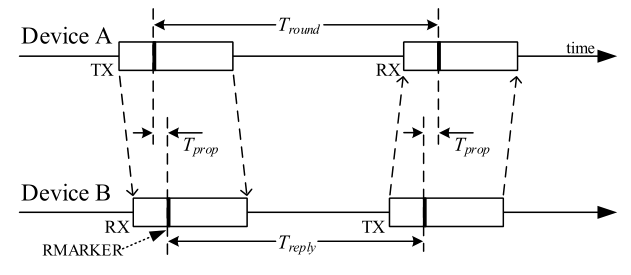
\includegraphics[width=\linewidth]{Figures/BasicRanging.png}
	\decoRule
	\caption{Single-sided two-way ranging. Figure from \parencite{DW1000UserManual}.}
	\label{fig:BasicRanging}
\end{figure}

In the case where there are two nodes communicating with each other, \parencite{DW1000UserManual} states that one can calculate the time it takes a signal to propagate between them, $T_{prop}$, as:

\[
	T_{prop} = \frac{T_{round} - T_{reply}}{2}
\]

where $T_{round}$ and $T_{process}$ are the total durations between receiving and transmitting messages as can be seen in Figure~\ref{fig:BasicRanging}.

\subsection{Double-sided Two-way Ranging}

\begin{figure}
	\centering
	\includegraphics[width=\linewidth]{Figures/AsyncRanging.png}
	\decoRule
	\caption{Double-sided two-way ranging with three messages. Figure from \parencite{DW1000UserManual}.}
	\label{fig:AsyncRanging}
\end{figure}

Because the clocks of two nodes may not pass time at the same rate (clock skew), the above equation will suffer from significant error. This is because processing times far dwarf the time it takes a signal to propagate. \parencite{DW1000UserManual} presents, without proof, the following equation for more accurate rangefinding:

\[
	T_{prop} = \frac{T_{round1}  T_{round2} - T_{reply1} T_{reply2}}{T_{round1} + T_{round2} + T_{reply1} + T_{reply2}}
\]

where $T_{round1}$, $T_{round2}$, $T_{reply1}$, $T_{reply2}$ are the durations between sending and receiving messages as seen in Figure~\ref{fig:AsyncRanging}. An independently derived proof of this equation can be found in Appendix~\ref{AsyncProof}.

Because the ranging has two rounds, after the initial calculation of range we can calculate a new range value for every single following transmission by re-using the last timestamps received for the beginning of the next round.

\section{Networking Basics}

Each node in the network broadcasts in a round robin fashion, with a small break after each node has transmitted. As part of the transmitted message, the node transmits the timestamp of when it is sending the message, a list of the timestamps when it last received a communication from every other node in the network, and a list of the last computed ranges to the other nodes. Every other node in the network will receive this information and use it to compute a new range to the node in question. Thus, every node in the network receives complete range information for the whole network.

The DWM uses 40 bits (5 bytes) for its timestamps. The Arduino internally represents these as 64-bit integers (the last byte being meaninless), but transmits them as 40 bit (5 byte) numbers.

Every node in the network has a pre-determined ID, which is set when it the code is programmed onto the device. A single byte is used for this ID to save as much space as possible, though the code could easily be modified to support longer IDs if the devices were to be mass produced. Alternately, something like DHCP could be implemented. As there are only 7 devices currently operational, our project only uses IDs 1 through 7, though the IDs do need not be consecutive. ID 255 is a special dummy value used in the code and should not be selected for use with an actual device.

Communications between the Arduino and the DWM1000 are handled through SPI. When the DWM1000 receives a message, it triggers an interrupt on the Arduino, which can then obtain the received data through SPI.

\section{Communications Timing}

\begin{figure}
	\centering
	\begin{tikzpicture}

\def \n {6}
\def \radius {3cm}
\def \margin {11} % margin in angles, depends on the radius

\begin{scope}[auto, every node/.style={draw,circle,minimum size=2em,inner sep=1},node distance=2cm]
\foreach \id [count=\s] in {1, 2, 5, 8, 10, 255}
{
  \node at ({360/\n * (\s - 1)}:\radius) {$\id$};
  \draw[->, >=latex] ({360/\n * (\s - 1)+\margin}:\radius) 
    arc ({360/\n * (\s - 1)+\margin}:{360/\n * (\s)-\margin}:\radius);
}
\end{scope}

\end{tikzpicture}
	\decoRule
	\caption{Transmission order of a network composed of five devices with IDs 1, 2, 5, 8, and 10. Note they transmit in order, and there is a dummy ID of 255 which serves as a marker for the end of the round.}
	\label{fig:TransmissionOrder}
\end{figure}

In order to maximize the operating frequency of the system and provide as smooth a visual experience as possible on the phone, we want to minimize the amount of time a node is not transmitting. In order to do this, it was decided that nodes should transmit in order of their ID in a round robin fashion. A round of transmissions are performed, each node transmitting once, and then it repeats. When one node receives a transmission, it checks to see if it is its turn and then transmits as soon as it can.

This round robin ordering is done by creating an ordered array of IDs in the network. When a transmission is received, the network increments the index of the next expected device to transmit by one. A device can tell whether it should transmit by checking to see if its ID is equal to the ID of the next expected node to transmit. If so, it transmits. 

The downside to this approach is that if any transmission were to be lost, for example by interference or electrical noise, the network would grind to a halt as it waits for a message that is never going to come. A solution to this is to include a timer that tracks a window in which a message should be received. If it takes too long to receive a message, the device was assumed to have to failed to transmit for some reason and the next device will take their turn and transmit.

To help the network be more robust, for example if one node has a clock that runs faster than the others (making it think a transmission is late when it is not), the network assumes whatever device last transmitted was right in doing so, and sets the index of the next node to transmit in the ordered array as being one higher than it.

This approach also raises the question of how new nodes will join the network if a node is constantly transmitting. To solve this, a small delay is added at the end of each round. When a device wishes to enter the network, it waits for the end of a round, and then does a transmission in this added space. This transmission lets all devices know it is part of the network, and they will add it to their ordered lists of IDs appropriately. 

In the code, this delay at the end of the round is implemented by adding a dummy node with the ID of 255 (the highest ID possible with one byte) to the network. The nodes will wait for a transmission from it at the end of each round, but it will never come, at which point the round starts over with the lowest ID transmitting. An example ordering can be found in Figure~\ref{fig:TransmissionOrder}.

An unsolved issue here is what happens when the transmission to join the network is sent and it is not received. This will cause the joining device to have a wrong order, and it will transmit at the same time as another device every round. Since the chances of this happening are quite low and could be solved by resetting the joining device, this is not dealt with. A possible solution to deal with this would be having the receiving device check the responses of all the other nodes to make sure they all received its transmission, and, if they have not, then to retransmit in the space at the end of the round until they do.

Code for this logic can be found in the \code{loop} function of Appendix~\ref{ArduinoCode}.

\section{Range Information Protocol}
The protocol for a transmission from a node is as follows:

\begin{itemize}
	\item 1 byte for the ID of the transmitting node.
	\item 5 bytes for the timestamp of the sending of the message.
	\item For each device the transmitting node has knowledge of:
	\begin{itemize}
		\item 1 byte for the ID of the device
		\item 1 byte for the shared counter (used to detect lost transmissions)
		\item 5 bytes for timestamp of last received message from the device
		\item 4 bytes for last calculated range	
	\end{itemize} 
\end{itemize}

Parsing a received message and updating range values from the parsed data is fairly straightforward. The code in question can be found in the \texttt{parseReceived} function in Appendix \ref{ArduinoCode}.

\section{Summary}
todo




% Rangefinding Hardware

\chapter{Rangefinding Hardware} % Main chapter title

\label{RangefindingHardware}

This chapter covers the specifics of the hardware and its use in the rangefinding subsystem. The topics covered are:
\begin{enumerate}
	\item The wireless communications technology used in the rangefinding subsystem, which is called ultra-wideband.
	\item Design justifications for the choice of the Decawave DWM1000 and Arduino Pro Mini chips.
	\item The design and construction of the anchors and tags used in the rangefinding subsystem, as well as the design of a PCB for the tags.
	\item A brief overview of how the DWM1000 is controlled in software.
	\item Performance metrics of the rangefinding subsystem.
\end{enumerate}

\section{Wireless Communications}
At the start of the project, it was determined that a technology would need to be chosen to handle wireless communications for ranging purposes. A number of options were considered. The ideal technology would:
\begin{itemize}
	\item Be inexpensive (a per-tag cost below \$100).
	\item Have a range exceeding 5m for in-door use.
	\item Allow for at least nanosecond-precision measurements of time. Due to the speed of light, a nanosecond of error in timing calculations would lead to approximately 30cm of error, so every nanosecond is significant.
	\item Be small (easily attachable to a standard Android phone).
\end{itemize}

Bluetooth was initially considered and explored for the wireless technology of the rangefinding subsystem, but it was found to not be appropriate for the project. Appendix~\ref{BluetoothFailure} goes into some details.

\subsection{Ultra-wideband and the DWM1000}
After doing some research, the Decawave DWM1000 ultra-wideband transceiver was discovered. The chip is advertised as specifically being suited for in-door ranging applications. It uses ultra-wideband technology rather than Bluetooth, Wi-Fi, or similar technologies.

\textbf{Ultra-wideband}, in contrast to Wi-Fi and other radio technologies, occupies a large bandwidth and transmits information via high-bandwidth pulses. Ultra-wideband is suited to in-door tracking applications due to how multipath propagation, a phenomenon where signals reflect off of surfaces and thus reach the antennae via multiple paths, enhances signal strength rather than causing interference as occurs in other radio technologies. 

An in-depth look at ultra-wideband is beyond the scope of this report.

The DWM1000 is advertised as:
\begin{itemize}
	\item Able to locate objects with up to 10cm accuracy,
	\item Having a range of up to 290m,
	\item Having a data rate of up to 6.8Mb/s,
	\item And having a small physical size. 
\end{itemize}

In addition, there was an already an open source library written to use the DWM1000 with an Arduino, which would allow us to quickly prototype with the chip and ensure it would be a good choice for the project.

Because these qualities satisfied our requirements, the DWM1000 was chosen for the foundational technology of the ranging part of the project. 

\section{Design of the Hardware}
The hardware design for tags is an Arduino Pro Mini 3.3V connected to a DWM1000 over a PCB. 

\subsection{The Microcontroller}
To interface with the DWM1000, a microcontroller was needed. The Arduino Pro Mini 3.3V was chosen because:
\begin{itemize}
	\item Others had used it with the DWM1000 and had good results \cite{LPSMini}.
	\item Members of Group 20 had previous experience with programming Arduinos.
	\item It was inexpensive (\$13 before tax).
	\item It worked off of 3.3V power, which was what the DWM1000 required. This obviated the need for voltage stepping.
	\item It was capable of floating point math, which is useful for calculating ranges. As well, barely any processing power or RAM was perceived to be needed. Each microcontroller only needed to hold a small number of timestamps, so the small amount of memory and slow processor was not important. (This was later discovered to be untrue.)
	\item It had a small physical size. As tags are attached to cellphones, they must be small.
	\item Batteries would not be needed to power tags, since power could be delivered via USB from the cellphone. This further simplified the design and kept costs low, though the USB cables required to connect the Arduinos ended up being quite expensive (\$22), mostly eliminating the cost savings.
\end{itemize}

The downside of the Pro Mini was that it required a lot of soldering. 

\subsection{Anchors}
\begin{figure}
	\centering
	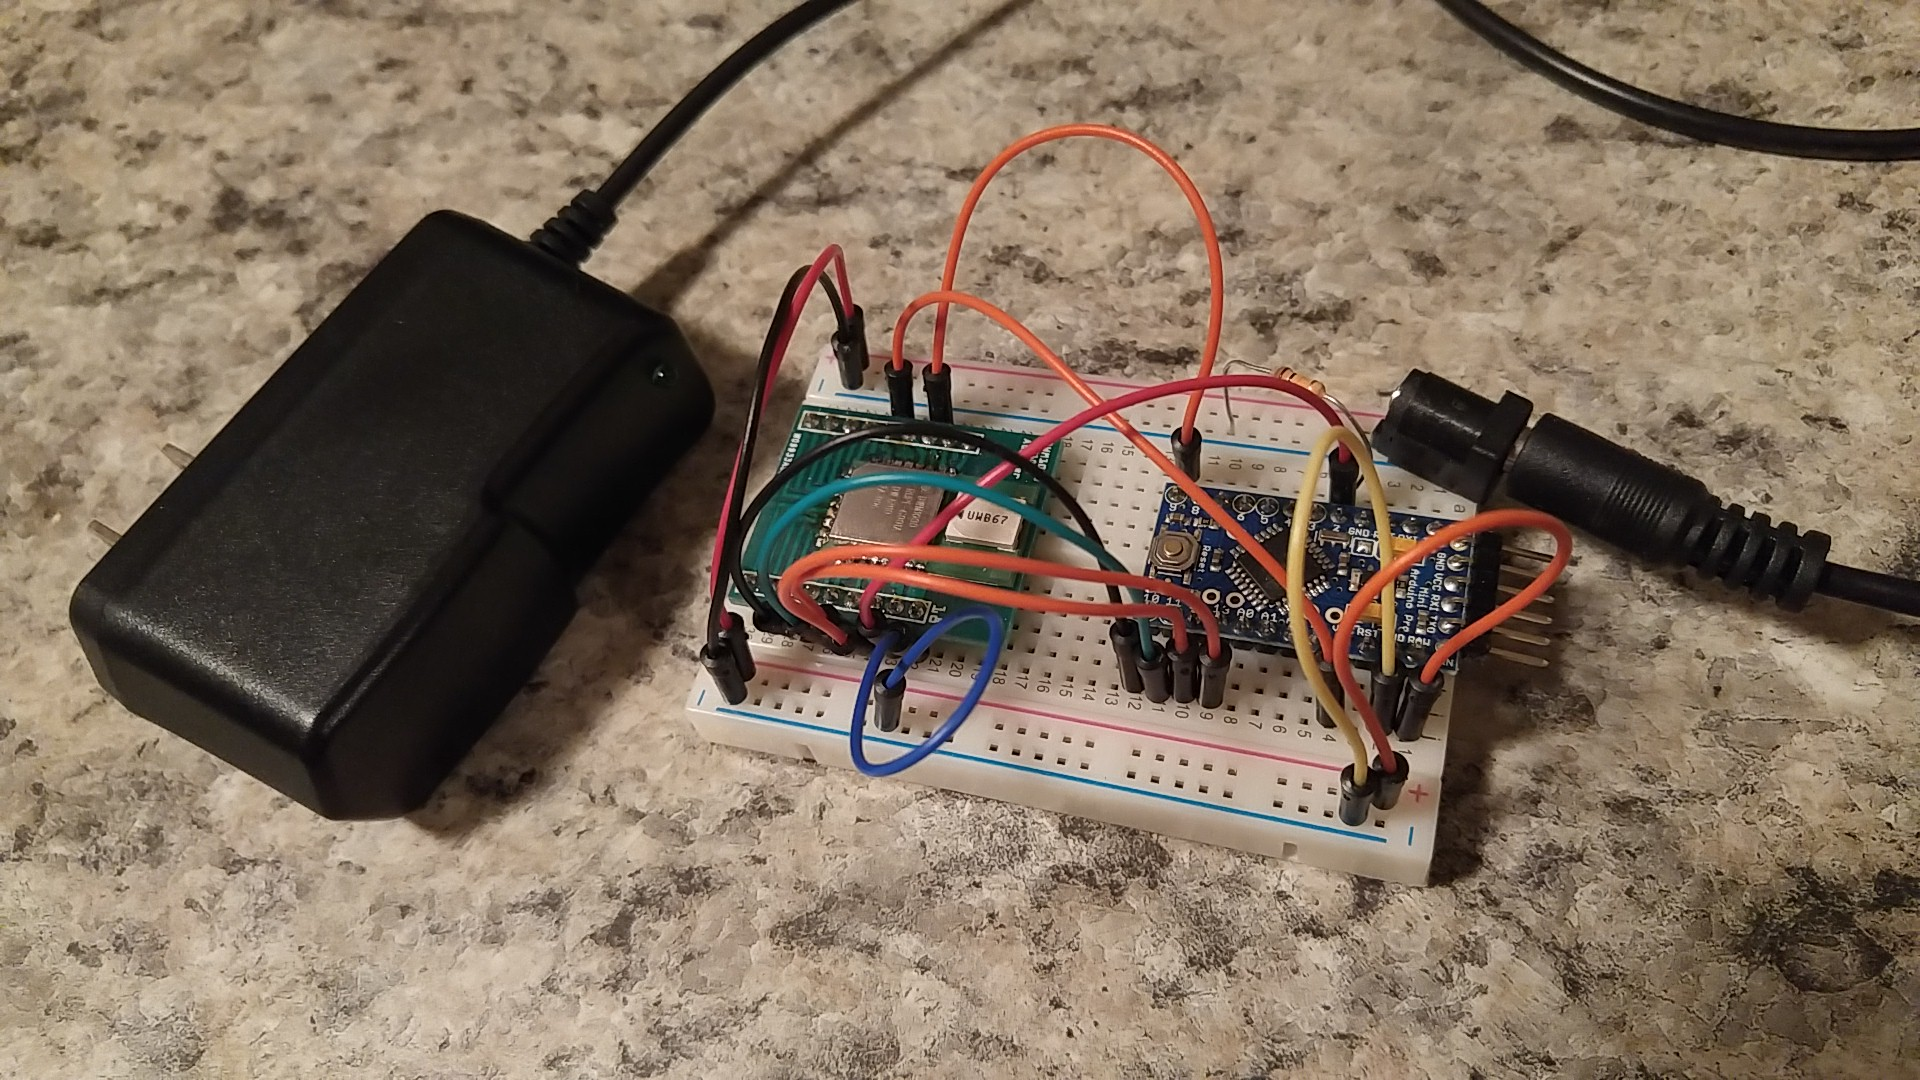
\includegraphics[width=\linewidth]{Figures/Anchor.jpg}
	\decoRule
	\caption{An anchor built on a breadboard using Thomas Trojer's PCB design \cite{ThotroGithub}. The DWM1000 is on the left, and the Arduino is on the right.}
	\label{fig:Anchor}
\end{figure}

The anchors made for use with this project were made on a breadboard and based on the design by Thomas Trojer in his \code{arduino-dw1000} library \cite{ThotroGithub}. A PCB design was included with this library which allowed a DWM1000 to be used with a breadboard. This PCB design was used in order to quickly prototype and determine whether the DWM1000 and Arduino would be feasible and meet the requirements for the project. Four anchors were constructed using these PCBs. An anchor can be seen in Figure~\ref{fig:Anchor}.

As anchors are assumed to be stationary, and the project is intended to be used in-doors, it was determined that the anchors could reasonably be powered via a standard electrical outlet. Designs using batteries were considered, but as the added flexibility in placement of the anchors considered to be marginal benefit (this later turned out to not be the case), and there was added complexity and maintenance required to deal with the batteries, using batteries as the power source of the anchors was not pursued.

To save costs and time, the anchors were not redesigned to be placed on a PCB, and instead remained mounted on breadboards. There was only marginal benefit to designing a PCB, as their size was mostly irrelevant and their performance would not be improved.

\subsection{Tags}
\begin{figure}
	\centering
	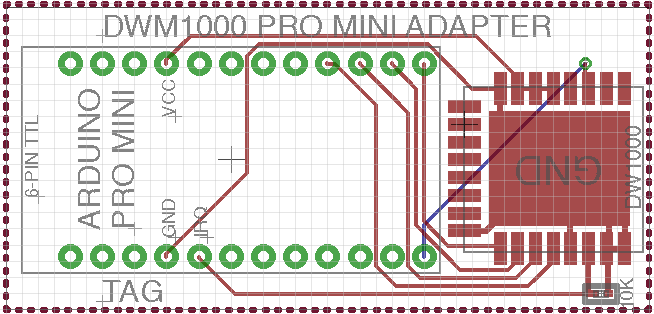
\includegraphics[width=\linewidth]{Figures/PCB.png}
	\decoRule
	\caption{The design for the tag PCB in EAGLE.}
	\label{fig:PCB}
\end{figure}

\begin{figure}
	\centering
	\includegraphics[width=\linewidth]{Figures/Tag.jpg}
	\decoRule
	\caption{A soldered tag.}
	\label{fig:Tag}
\end{figure}
The tags made for use with this project were required to be small enough to comfortably attach on a headset or cellphone. As the breadboards were too large, a custom PCB was designed.

Several designs were considered for the PCB connecting the Arduino and DWM1000. The most important factors were size and cost.

Several designs were considered at first:
\begin{itemize}
	\item The first idea considered was to place the Arduino and DWM on top of each other, resulting in the smallest possible size. However, the physical dimensions of the two components made this impossible. Pins from each component would have to be laid on each other, resulting in a circuit that does not work.
	\item Another possibility was to place each component on opposite sides of the PCB, but the Arduino's design demanded breakout headers to solder it into the board, which meant the PCB had to have holes drilled, which again meant that the physical dimensions of the two components interfered.
	\item Yet another idea was to make two PCBs. The Arduino would connect to a PCB above it, and that PCB would connect to a board above it with the DWM1000 soldered to it. Because it was layered, the pins connecting the layers could be arranged such that the Arduino and DWM1000 were essentially above each other, but without the locations of their pins interfering with each other. This design was abandoned because the breakout pins would add a large amount of vertical length, it was twice as expensive, and because it was much more complex to design.
	\item The final idea considered was to have the Arduino and DWM1000 just be placed next to each other on the same side of a PCB. This design was physically realizable, the least expensive, and though it was not as compact as would be ideal, it was still small enough to meet the requirements.
\end{itemize}

The last idea was chosen due to the its cheap cost, simplicity of design, and satisfactory size. 

As others who had used the DWM1000 recommended it \cite{LPSMini}, the PCB was designed so the antenna would not be on the PCB.

The PCB design was done in EAGLE and ordered from PCBWay. The PCB design can be seen in Figure~\ref{fig:PCB} and a soldered tag can be seen in Figure~\ref{fig:Tag}.

\section{Arduino Software}
The software to control the DWM1000 was written in C++ in Arduino IDE. The basic code to control the DWM1000 (handling memory address constants, communication with it via SPI, and a few high-level functions like send/receive) was available in Thomas ``thotro'' Trojer's open-source \code{arduino-dw1000} library. The library served as the foundation of the code used in this project to network the tags and anchors.

\subsection{Calculating a Delay}
\label{CalculatingADelay}
As part of the time-of-flight calculation, a timestamp is needed for when the ranging message was received and for when the reply was sent. The DWM1000 does not offer a way to automatically set the time upon transmission, but does offer the ability to set a time when a message will be transmitted in the future. If a delayed transmission is sent, the timestamp can be calculated ahead of time and then be embedded in the message.

Ideally, this delay is short. However, if the delay is too short, the Arduino will not be able to transmit the message data to the DWM1000 before the delayed timestamp is passed. This causes a silent error, and the DWM will not transmit anything. As well, the delay specified is not quite the delay at which the DWM1000 will begin transmitting, it is the delay that the DWM1000 will begin transmitting the data portion of the message. There is a ``premable'' sent before any transmission to allow the other devices in the network time to wake up and learn that a message is coming. Sending the preamble takes a relatively long time (approximately 1 microsecond per symbol in the preamble, which adds up to almost 2 ms for the preamble length chosen for this project). This was the most difficult to solve bug that was encountered in the design of the system.

The delay before a node can transmit is the sum of the:
\begin{itemize}
	\item Number of symbols in the preamble $\times$ 1\si{\micro\second} (2048 is the value used here, though the DWM offers different choices of preamble length, it is not exactly 1 \si{\micro\second} but it is very close)
	\item Time required to calculate and send the timestamp using SPI, about 1000\si{\micro\second} (empirically determined)
	\item Bytes of data to transmit $\times$ 4.5\si{\micro\second}, or 85 $\times$ number of devices in the network besides this one (empirically determined)
\end{itemize}

Adding in a fudge factor of about 200\si{\micro\second}, the delay we use in code for 6 devices is roughly 3500 \si{\micro\second}.

It is important to minimize this delay so as to increase the maximum frequency the system can update ranges at. The tradeoff of having a short preamble versus a long one is that a longer preamble takes time to send, but has a lower probability of being missed by the recipients. Tests indicated that the longest preamble, 2048 symbols, would be useful for in-door ranging due to the number of obstructions which would interfere with signals.  Shorter preambles resulted in missed messages a longer preamble could send without difficulty.

\section{Calibrating}
DWM1000s need to be calibrated to give correct distances due to the capacitance of the hardware connected to the chips, among other factors. Some of these factors are controlled for in software in the \code{arduino-dw1000} library. For a detailed overview of the possible errors and how to correct for them, the reader is advised to read the relevant sections in the DW1000 User Manual \cite{DW1000UserManual}.

The primary factor which could not be controlled for by the manufacturer, Decawave, was the antenna delay. The capacitance of the hardware the DWM1000 is hooked up to can cause nanosecond-level delays in transmission (in experiments, it was found that this could cause a meter of error or more incorrectly configured). This is a constant, and is determined empirically. The antenna delay constant for the tags is roughly the same. Accurate values (under 50cm of error) were in the range of 16470-16500, and the antenna delay for the anchors is roughly the same and was found to be INSERT NUMBER HERE TODO.

Changing the antenna delay in the main code for easier calibration required changes to the \code{arduino-dw1000} library. A link to the code can be found in Appendix~\ref{ArduinoCode}.

\section{Results}
\label{RangefindingResults}
Results showed that the DWM1000 was close to as accurate as Decawave claimed (under 10cm). The project was found to be within 50cm most of the time, and it is possible more calibration could have improved this further). However, sometimes the reported ranges would glitch and be off by a meter or more. Table~\ref{tab:RangefindingAccuracy} shows the accuracy of the system. Though the accuracy of the rangefinding system was not a direct requirement of the project as a whole, the accuracy of the rangefinding system translates into accuracy of the position calculating system and thus the accuracy of the markers on the AR display.

\begin{table}
\caption{Accuracy of the rangefinding subsystem. Experiment performed with a tape measure and two tags lying on the hardwood floor of an apartment. Antenna delay 16470.}
\label{tab:RangefindingAccuracy}
\centering
\begin{tabular}{c c c}
\toprule
\tabhead{Actual Distance (m)} & \tabhead{Mean Reported Distance (m)} & \tabhead{Standard Deviation (m)} \\
\midrule
0.5 & 0.62 & 0.045 \\
1 & 1.08 & 0.025 \\
2 & 2.24 & 0.03 \\
3 & 3.21 & 0.022 \\
4 & 4.22 & 0.104 \\
\bottomrule 
\end{tabular}
\end{table}

The operating frequency was close to the values predicted by theory, as can be seen in Appendix~\ref{OperatingFrequencyAnalysis}. Frequency values can be found in Table~\ref{tab:RangefindingFrequency}.

The max range between nodes was not determined due to space limitations but was at least 10m. The DWM1000 User Manual claims that the there is at least 60m of range if there are no obstructions \cite{DWM1000UserManual}.

\begin{table}
\caption{The frequencies of the rangefinding subsystem for various numbers of devices in the network. Experimented performed by placing an increasing number of devices in a network and calculating the duration between range reports from node 1 to node 2.}
\label{tab:RangefindingFrequency}
\centering
\begin{tabular}{c c c}
\toprule
\tabhead{Number of Devices} & \tabhead{Round Time (\si{\micro \second})} & \tabhead{Frequency (Hz)} \\
\midrule
2 & 37000 & 27 \\
3 & 58000 & 17.2 \\
4 & 86000 & 11.6 \\
5 & 93000 & 10.8 \\
6 & 156000 & 6.4 \\
7 & 170000 & 5.9 \\
\bottomrule
\end{tabular}
\end{table}

\section{Summary}
This chapter covered ultra-wideband, the wireless communications technology used in the rangefinding subsystem, and how it is particularly well suited to in-door rangefinding applications. 

Reasons for why the DWM1000 and Arduino Pro Mini were discussed. The DWM1000 was known to be suitable for this application, and the Arduino Pro Mini was known to have software already written for it to interface with the DWM1000.

The design of the tags and anchors was discussed. Tags had custom PCBs designed for them due to their need to be a small size, while anchors were kept on a breadboard because there was no advantage to resoldering them on a PCB.

The code used to control the DWM1000 was brought up. It is particularly important to keep in mind how long the Arduino takes to process messages, as delayed messages are used to transmit the timestamp of when a message is sent, and if the Arduino takes too long the message will fail to send.

Finally, performance metrics were discussed. The system can determine ranges with an accuracy of under 50cm, and can update ranges 5.9-27Hz depending on how many devices are in the network.


% Position Calculation


\chapter{Position Calculation} % Main chapter title

\label{PositionCalculation}

%----------------------------------------------------------------------------------------

\section{Overview}
%Talk about the goal of this section: to calculate positions of objects given the ranges between them. Talk about how Arduinos and Androids are connected by FTDI.

Our location tracking system consists of two different anchors, anchors and tags. The anchors which we can think of as static anchors doing the postion tracking, and the tags which are our dynamic anchors that we need to track. The overall goal of this subsystem is to calculate the position of each anchor given only the distances from one another.
The anchors use ultrawideband technolgy to communicate with each other and send the position data to our android application using FTDI.


\section{High-Level Example in 2D}
To start the position calculation we take three different anchors for example $a_{0}$, $ a_{1}$  and $a_{2}$. We set an arbitrary point as the origin $a_{0}$, then we proceed to make a horizontal line from $a_{0}$ to another anchor say $a_{1}$, since we have all the distances between the anchors we can now use basic trigonometry to calculate the position of our last anchor $a_{2}$.
An Example calculation is as follows:
\\\\
distance from anchor x to anchor y: $d_{xy}$, we use cosine law to determine the angle
\\
\[ \Theta = \cos ^{ - 1}\Big(\frac{d_{01}^2 + d_{02}^2 - d_{12}^2 }{2*d_{01}*d_{02}}\Big)\]
\\
when we have the angle we can now calculate the x and y coordinates:
\\
\[ x_2 = cos(\Theta) * d_{12} \]
\[ y_2 = sin(\Theta) *  d_{12} \]

\section{Extending This to 3D}
Extending the subsystem to three dimensions does not really change the calculation all that much except that we now need four anchors to get a reliable position in three dimensions. We have our four anchors: $a_{0}$, $a_{1}$ , $a_{2}$ and $a_{3}$, we arbitrarily set one as the origin $a_{0}$(0, 0, 0) and we now make a horizontal line to another anchor say $a_{1}$ and since we know the distance between these two anchors we can get the position to be $a_{1}$(0, $d_{01}$, 0), where $d_{01}$ is the distance between $a_{0}$ and $a_{1}$. We can now form a triangle with the third anchor and use cosine law to determine the position and we arbitrarily set the z value to 0.
\\
We now have the coordinates for the third anchor, but we do not know the correct orientation in the z axis, it could be either positive or negative. This is where the fourth anchor comes in, we use the anchor to create a temporary point using the same method we use above.
\\
\[ \Theta = \cos ^{ - 1}\Big(\frac{d_{01}^2 + d_{03}^2 - d_{13}^2 }{2*d_{01}*d_{03}}\Big)\]
\\
\[ x_{temp} = cos(\Theta) * d_{13} \]
\[ y_{temp} = sin(\Theta) *  d_{13} \]
\[ z_{temp} = 0 \]
\\
We will rotate around the x-axis by keeping the x value constant and taking the y distance and z distance to be a circle of radius of $y_{temp}$.We calculate the distance between the x value of the temporary point and the x value of anchor 2, we denote this value $\Delta x$.
\\
\[ \Delta x = x_{temp} - x_{2} \]
\\
Now that we have $\Delta x$ we can now calculate the position of our fourth anchor using cosine law.
\\
\[\Theta = \cos ^{ - 1}\Big(\frac {\Delta x^2 - d_{23}^2 + y_{2}^2 + y_{temp}^2}{2*y_{2}*y_{temp}}\Big)\]
\\
\[ x_{3} = x_{temp} \]
\[ y_{3} = cos(\Theta) * y_{temp} \]
\[ z_{3} = sin(\Theta) * y_{temp} \]


\section{Arbitrariness (pick a better title later)}
The positions calculated from ranges do not correspond to the real world! We must use the cellphones' accelerometer (for gravity) and magnetic sensor (for compass direction/inclination) to map these positions to reality.

Go over how this is done.

\section{Getting the Ranges}
Talk about FTDI and our protocol to communicate from Arduino to Android. Go over how they are parsed (put in appendix of parsing code)

\section{Conclusion}
This subsystem calculates positions; we figured out how ranges are obtained, how they are calculated. Go over this in more detail.
% Augmented Reality

\chapter{Augmented Reality} % Main chapter title

\label{AugmentedReality}

%----------------------------------------------------------------------------------------

This chapter covers the AR portion of the project. The AR subsystem takes the positions from the position calculation subsystem and renders them on the screen. If they cannot be directly rendered, an arrow is drawn on the edge of the screen to show which way the object is from the user. An example of this can be found in Figure~\ref{dfis} (DO THIS FIGURE).

The code for the AR subsystem can be found at (PROVIDE LINK HERE).

This chapter covers the following topics:
\begin{enumerate}
	\item A description of OpenGL and the basics of how it can be used. 
	\item A brief overview of the math used later in this section, including homogenous coordinates and translation/rotation matrices.
	\item How objects and text can accurately be drawn on the screen overlaid on a camera image.
	\item How the coordinate system of the position calculation system can be transformed into real world coordinates through the cell phone's sensors.
	\item Examples of the accuracy of the subsystem.
\end{enumerate}

\section{OpenGL}
Go over OpenGL, the 3D text rendering library we're using, Android's rotation calculations.

\section{Projection, View, Model Matrices}
maybe put this below

\section{3D Math Overview}
This section covers the basics of using matrices to render 3D scenes. A full treatment of the subject is beyond the scope of this report, though other resources on the subject exist (PUT CITATION HERE).

\subsection{Rotation Matrices}

\subsection{Homogenous Coordinates}
For a given 3$\times$3 matrix $M$ and an arbitrary point in 3D space $p = (x, y, z)$, there is no $\mathbf{M}$ such that will multiplying it by any $p$ will cause $p$ to be translated by a specified number of units. There is, however, a way to do it with a homogenous point and a 4x4 matrix. This is one of the reasons homogenous coordinates are used in OpenGL.

Homogenous coordinates are coordinates in space which contain an extra element $w$ which acts as a scaling factor on the three elements. For example, a 3D homogenous coordinate $p_h$ could be written as:

\[ p_h = (x_h, y_h, z_h, w) \]

This relates to a regular point in 3D space:

\[ (x, y, z) = (x_h / w, y_h / w, z_h / w) \] 

For example, the homogenous point $(1, 1, 1, 1)$ maps to the regular 3D point $(1, 1, 1)$. The homogenous point $(2, 2, 2, 2)$ does as well.

A translation matrix $T$ that moves a point $p$  by $(T_x, T_y, T_z)$ units, is:

\[
\mathbf{T} = \begin{bmatrix}
1 & 0 & 0 & T_x \\
0 & 1 & 0 & T_y \\
0 & 0 & 1 & T_z \\
0 & 0 & 0 & 1
\end{bmatrix}
\]

To prove this, we'll multiply out a homogenous point $p_h = (x_h, y_h, z_h, w)$ by $\mathbf{T}$ and show that, when converted to a regular 3D point, it equals $(x/w + T_x, y/w + T_y, z/w + T_z)$.

\[ p_{h}\prime = \mathbf{T} p_h \]

\[
  p_{h}\prime = \begin{bmatrix}
1 & 0 & 0 & T_x \\
0 & 1 & 0 & T_y \\
0 & 0 & 1 & T_z \\
0 & 0 & 0 & 1
\end{bmatrix} 
\begin{bmatrix}
x_h \\ y_h \\ z_h \\ w 
\end{bmatrix}
\]

\[
 p_{h}\prime = \begin{bmatrix}
 x_h + w T_x \\
 y_h + w T_y \\
 z_h + w T_z \\
 w
 \end{bmatrix}
 \]
 
 Now, if we convert $p_{h}\prime$ to a regular 3D point $p$, we get:
 
 \[ p = (\frac{x_h}{w} + \frac{w T_x}{w},  \frac{y_h}{w} + \frac{w T_y}{w}, \frac{z_h}{w} + \frac{w T_z}{w}) \]
 \[ p = (x/w + T_x, y/w + T_y, z/w + T_z) \]
 
 which is the translation of $p$ by $(T_x, T_y, T_z)$ units.

\section{Camera Field of View and OpenGL Field of View}
Talk about how we make positions accurate here. Go over how we just overlay the camera and OpenGL surface on each other. Discuss Android camera limitations/FPS results.

\section{Cellphone Rotation}
Discuss in detail more about how Android implements getting the rotation, the limits of it when moving + in strong magnetic fields.

\section{Billboard Effect}
Talk about how doing the inverted view matrix multiplication causes things to always face the screen. Give pictures! Motivation here is to make 2D images that we can place in 3D space and have them face the screen.

\section{HUD}
Go over how the HUD is made. (Still need to finish that too so we can get pictures.)

\section{Calibration}
Talk about how we can take the cellphone's rotation matrix and calibrate the positions we calculate from anchors/tags.

\section{Results}
Show off how accurate we are. Have Youtube videos displaying such.

\section{Conclusion}
Conclusion of this section: we can render positions on the screen and have 3D math to do so etc.

% Conclusion

\chapter{Conclusion} % Main chapter title

\label{Conclusion} % For referencing the chapter elsewhere, use \ref{Chapter1} 

%----------------------------------------------------------------------------------------

The project shows that with much more refinement, a practical application of augmented reality is closer to reality than previously envisioned. The project is operating on a device that can be easily obtained by the average consumer. While devices such as the HTC Vive and Occulus Rift demonstrate the power of virtual reality and the potential to be augmented in real life, it is currently out of the practical price range of many consumers. Most of the time, a user will also require a powerful personal computer to run the programs, which can range at least one thousand dollars. Google Cardboard shows that with an Android device virtual reality can be experienced more cheaply, except for the tags which must be obtained on top of the Android device. 

There are three main topics that were covered in this report: augmented reality rendering, position calculation and range finding. Distances between devices are determined via ultra-wideband transceivers using time-of-flight calculations. These distances are then used to calculate positions of the objects in 3D space. Finally, these positions are rendered on the screen with the augmented reality subsystem.

The system is able to accurately display the locations of tracked objects to under 50 cm at distances over 10 meters, and provide updates to their positions at over 4Hz.

A HUD has been realized outside of videogamesl. The applications of the techniques in this report are numerous. They can range from surgeons knowing the status of their patient, location tracking, and more immersive entertainment. 

\section{Future Work}
A number of aspects of work on the project were left incomplete due to time constraints. They offer paths for future work to focus on:

\begin{enumerate}
	\item An integrated GPS location could be included that would display the locations of GPS coordinates on the display relative to your current GPS coordinates.
	\item The Arduino Pro Mini could be upgraded with a faster microcontroller which could improve the system operating frequency by an order of magnitude.
	\item The anchors could have PCBs designed for them.
	\item An automatic calibration system could be designed that such that the user does not have to manually calibrate the system on startup. The system would use dead reckoning and the velocity of the user as measured by the position calculation system to determine a rotation matrix to calibrate the system.
	\item A more powerful mathematical technique for calculating positions in 3D space could be used which takes in the extra range data that the tags have to each other. This could be used to minimize error and filter out noise.
\end{enumerate}

%----------------------------------------------------------------------------------------
%	THESIS CONTENT - APPENDICES
%----------------------------------------------------------------------------------------

%\appendix % Cue to tell LaTeX that the following "chapters" are Appendices

% Include the appendices of the thesis as separate files from the Appendices folder
% Uncomment the lines as you write the Appendices

\begin{appendices}
% ArduinoCode

\chapter{Source Code} % Main appendix title
\label{SourceCode} % For referencing this appendix elsewhere, use \ref{AppendixA}

This appendix lists all the code used in the project. The project names are named according to their function.

\section{AR Code}
All of the Android application code is packaged in \code{ARLocationTracking}. It also contains code to handle the rendering
of pointers and texts on the screen, as well as code allowing the phone to communicate
with the Arduino chips via FTDI and USB. A modified version of the Texample23D open source project, used for rendering text in 3D, is included in the project. The modifications allow the 3D text to be rotated with an arbitrary matrix. This is used to billboard the rendered text. Finally, the EAGLE schematics for the tags' PCB is contained within this project. The project can be found at \url{https://github.com/DrewBarclay/ARLocationTracking}.

\section{Arduino Code}
In \code{dw1000arduinonetwork} is all of the code that runs on the Arduinos. It contains all of the code necessary
to interface with the DWM1000 and form a network. This package does not contain any position calculation code; that can be found in \code{TagParser.java} in the AR Code. The project includes a modified version of the \code{arduino-dw1000} project by Thomas Trojer. The modifications allow the easy setting of antenna delay from the main Arduino code. The code can be opened and compiled in Arduino IDE. Arduino IDE must be configured to compile C++ code. The project can be found at \url{https://github.com/DrewBarclay/dw1000arduinonetwork}.


% AsyncProof

\chapter{Asynchronous Two-Way Ranging Proof} % Main appendix title

\label{AsyncProof} % For referencing this appendix elsewhere, use \ref{AppendixA}

\begin{figure}
	\centering
	\includegraphics[width=\linewidth]{Figures/AsyncRanging.png}
	\decoRule
	\caption{Double-sided Two-way ranging with three messages\cite{DW1000UserManual}.}
	\label{fig:AsyncRangingAppendix}
\end{figure}

We begin by assuming that the clock of one node is off by alpha ($\alpha$) and the other by beta ($\beta$), the key here was to find the time of flight in a virtual clock that would be the mean value of alpha and beta.
\\
\[ \alpha a = 2t + \beta c  \tag{1} \label{eq:1} \]
\[ \beta d = 2t + \alpha b  \tag{2} \label{eq:2} \]
\[ 1 = \frac{\alpha + \beta}{2} \]
\\
We simplify and solve for $\beta$:
\\
\[ \beta = 2 - \alpha  \tag{3} \label{eq:3} \]
\\
We then subsititute equation \eqref{eq:3} into equation \eqref{eq:1} and equation \eqref{eq:2}.
\\
\[ \alpha a = 2t + 2c - \alpha c  \tag{4} \label{eq:4} \]
\[ 2d - \alpha d = 2t + \alpha b  \tag{5} \label{eq:5} \]
\\
Isolate $\alpha$ for both equations \eqref{eq:4} and \eqref{eq:5} we get the following:
\\
\[ \alpha = \frac{2(t + c)}{a + c}  \tag{4.1} \label{eq:4.1} \]
\[ \alpha = \frac{2(d - t)}{b + d}  \tag{5.1} \label{eq:5.1} \]
\\
Setting \eqref{eq:4.1} and \eqref{eq:5.1} equal to each other we can solve for propagation time, t.
\\
\[ 2(t + c)(b +d) = 2(d - t)(a + c)\]
\[ tb + td +bc + dc = da + dc - ta - tc \]
\[ t(b + d + a + c) = da - bc\]
\[ t = \frac{da-bc}{a + b + c + d}  \tag{6} \label{eq:6} \]
\\

%\include{Appendices/AppendixB}
%\include{Appendices/AppendixC}
\end{appendices}

%----------------------------------------------------------------------------------------
%	BIBLIOGRAPHY
%----------------------------------------------------------------------------------------

\printbibliography[heading=bibintoc]

%----------------------------------------------------------------------------------------

\end{document}  
